\documentclass[modern]{aastex631}
%\documentclass[twocolumn]{aastex631}

\usepackage{amsmath}
\usepackage{soul}

% Abundance and stellar macros
\newcommand{\mgfe}[0]{[{\rm Mg/Fe}]} 
\newcommand{\afe}[0]{[\alpha/{\rm Fe}]}
\newcommand{\femg}{[{\rm Fe}/{\rm Mg}]} 
\newcommand{\xmg}{[{\rm X}/{\rm Mg}]} 
\newcommand{\mgh}{[{\rm Mg}/{\rm H}]}
\newcommand{\feh}[0]{[{\rm Fe/H}]} 
\newcommand{\xfe}{[{\rm X}/{\rm Fe}]} 
\newcommand{\xh}{[{\rm X}/{\rm H}]} 


\newcommand{\logg}{\log(g)}
\newcommand{\teff}{T_{\rm eff}}
\newcommand{\kpc}{\rm \; kpc}
\newcommand{\kel}{\rm \; K}
\newcommand{\msun}{M_{\odot}}
\newcommand{\rgc}{R_{\rm GC}}
\newcommand{\msunvice}{M_{\odot}/M_{\odot \rm formed}}
\newcommand{\MZAMS}{M_{\rm ZAMS}}

\newcommand{\qcc}{\vec{q}_{{\rm CC,}j}^{Z}}
\newcommand{\qccFe}{\vec{q}_{{\rm CC, Fe}}^{Z}}
\newcommand{\dqccFe}{d\vec{q}_{{\rm CC, Fe}}^{Z}/dZ}
\newcommand{\qIa}{\vec{q}_{{\rm Ia,}j}^{Z}}
\newcommand{\qIaFe}{\vec{q}_{{\rm Ia,Fe}}^{Z}}
\newcommand{\Acc}{A^{\rm CC}_{i}}
\newcommand{\AIa}{A^{\rm Ia}_{i}}
\newcommand{\fcc}{f_{\rm CC}}



\newcommand{\ejg}[1]{\textcolor{red}{EJG: #1}}

%% Reintroduced the \received and \accepted commands from AASTeX v5.2
%\received{March 1, 2021}
%\revised{April 1, 2021}
%\accepted{\today}

%\submitjournal{ApJ}

\newcommand{\name}{\textsl{Foo}} % Hogg's just making this up; change it!!
\newcommand{\documentname}{\textsl{Article}}

\shorttitle{data-driven few-process model for nucleosynthesis}
\shortauthors{griffith and hogg}
\addtolength{\topmargin}{-0.4in} % trust in Hogg
\addtolength{\textheight}{0.7in} % trust in Hogg
\setlength{\parindent}{1.6em}
\renewcommand{\paragraph}[1]{\bigskip\par\noindent{\textbf{#1}}~---}
\sloppy\sloppypar\raggedbottom\frenchspacing % Trust Hogg

\graphicspath{{./}{Figures/}}
\begin{document}

\title{\name: A data-driven few-process model for nucleosynthesis}

\correspondingauthor{Emily J. Griffith}
\email{Emily.Griffith-1@colorado.edu}

\author[0000-0001-9345-9977]{Emily J. Griffith}
\altaffiliation{NSF Astronomy and Astrophysics Postdoctoral Fellow}
\affiliation{Center for Astrophysics and Space Astronomy, Department of Astrophysical and Planetary Sciences, University of Colorado, 389~UCB, Boulder,~CO 80309-0389, USA}

\author[0000-0003-2866-9403]{David W. Hogg}
\affiliation{Center for Cosmology and Particle Physics, Department of Physics, New York University, 726~Broadway, New~York,~NY 10003, USA}
\affiliation{Max-Planck-Institut f{\"u}r Astronomie, K{\"o}nigstuhl 17, D-69117 Heidelberg, Germany}
\affiliation{Flatiron Institute, 162 Fifth Avenue, New~York,~NY 10010, USA}

% \author[0000-0001-7775-7261]{David H. Weinberg}
% \affiliation{The Department of Astronomy and Center of Cosmology and AstroParticle Physics, The Ohio State University, Columbus, OH 43210, USA}
% \affiliation{The Institute for Advanced Study, Princeton, NJ, 08540, USA}

\begin{abstract}\noindent % trust Hogg

\ejg{Need to update abstract}

Stellar surface abundances look like they are produced by two dominant processes, one prompt and one delayed.
We analyze YYY abundance ratios (ratioed to Mg) for XXXX stars from APOGEE DR17 with a flexible two-process model, in which all element process amplitudes are free parameters.
The two-process model describes each element abundance of each star as the vector sum of a CCSN and SNIa process.
Prior work derives process amplitudes from median observed high-Ia and low-Ia abundance trends; we relax these assumptions and simultaneously fit all model parameters to the data, with only minimal constraints to keep the processes interpretable.
We compare fit parameters from this new method to those derived from prior work [that the two methods produce similar results but with XXX differences and identify similar outlier stars??].
Our flexible method---dubbed \name---tests the validity of the standard two-process assumptions, such as Mg being a pure CCSN element, and that Solar abundances are generated by a roughly half-half combination of CCSN and SNIa processes.
We find [that the assumptions of prior work are generally confirmed. But that the inferred Fcc value of Fe peak elements is strongly dependent upon the chosen CCSN process strength for Fe].
We capitalize on the flexibility to explore the addition of a third process, agnostic about its origin.
The third process most improves [X elements? most significant for X elements?].
Most importantly, \name{} can be extended to populations at very low metallicity, and populations without two clear abundance sequences, such as the LMC/SMC, Sagittarius, and Gaia-Enceladus (??), making it a general diagnostic for enrichment; in principle, it can also be used to constrain fundamental nucleosynthetic parameters.
\end{abstract}

\keywords{foo --- bar}

\section*{}\clearpage
HOGG SAY: Here are some things to do or think about:
\begin{itemize}
  \item Should we think of this as a 2-process model or as a $K$-process model, where $K$ is often 2? I'm leaning towards $K$.
  \item \ejg{I like the K-process model. (This is named $N$-Process model in W22)}
  \item What are we going to do in terms of interpreting the results? These process vectors aren't exactly yields; they are something way more complicated, right?
  \item \ejg{Interpret in terms of $\fcc$. Can also make inferences about the metalicity dependence of SNIa/CCSN enrichment to given elements based on how $\qcc$ and $\qIa$ evolve with time.}
\end{itemize}

\section{Introduction}\label{sec:intro}

After hydrogen, helium, lithium, and beryllium, essentially all other naturally occurring elements are made in stars, and the collisions of stars.
%We are literally made of star stuff.
Stellar surface abundances---the abundances measured by taking a spectrum of a stellar photosphere---are thought to deliver a relatively unprocessed (for most elements) record of the element abundances in the gas from which the star formed (though see \ejg{Add citations}).
These birth abundances were set by a combination of nucleosynthetic processes involved in making heavy atomic nuclei, and astrophysical processes involved in delivering atoms from stellar interiors to star-formation sites \citep[e.g.,][]{johnsonja2020}.
Thus nuclear physics and a wide swath of astrophysics are critically intertwined in our understanding of stellar surface abundances, motivating theoretical, experimental, and observational work.

At the present day, stellar surface abundances are not very well explained by \textsl{ab initio}, physics-driven models.
Yields vary from set to set, as they are dependent on progenitor properties and explosion assumptions \citep[e.g.,][]{rybizki2017, griffith2021b}. 
The wide parameter space of progenitor and supernovae models coupled with uncertainties in reaction rates and explosion physics hinder the creation of an accurate nucleosynthetic model from theory alone.
In the long run, it is incumbent upon us to understand these issues and correct the assumptions or calculations underlying our nucleosynthetic and astrophysical models.
In the short run, however, we gather data---tens of millions of abundance measurements on millions of stars in different astronomical surveys such as RAVE, SEGUE, LAMOST, Gaia-ESO, APOGEE/MWM, GALAH, and H3 \citep{steinmetz2006, yanny2009, gilmore2012, desilva2015, luo2015, majewski2017, conroy2019}.
This raises the question: \emph{Can we take a data-driven approach to nucleosynthesis?}

In this \documentname{}, we build a purely data-driven model for the surface element abundances observed in stars.
We treat each star as being a linear combination of nucleosynthetic processes, beginning with one that is primarily responsible for the $\alpha$-element Mg \citep[core collapse supernovae (CCSN), e.g.][]{andrews2017}, and one that is primarily \emph{not} (Type-Ia supernovae (SNIa)).
Beyond that up-front assumption, we try to be agnostic about how the elements are produced.

We build upon the work of \citet[][hereafter G22]{griffith2019, griffith2022} and \citet[][hereafter W22]{weinberg2019, weinberg2022}, who used the bimodality in [Mg/Fe] vs. [Fe/H] \citep[e.g.,][]{fuhrmann1998, bensby2003, adibekyan2012} to separate stars into populations with high and low SNIa enrichment. Using the median [X/Mg] vs. [Mg/H] abundance trends, these works explain data from the \textsl{GALAH}\footnote{GALAH = GALactic Archaeology with HERMES.} and SDSS-IV \textsl{APOGEE}\footnote{APOGEE = Apache Point Observatory Galactic Evolution Experiment, part of the Sloan Digital Sky Survey} surveys, respectively, with a two-process model. Because the median abundance trends in [X/Mg] vs. [Mg/H] space are largely insensitive to aspects of chemical evolution, such as outflows and variations in star formation history \citep{weinberg2019}, the population abundance trends are set by the nucleosynthetic processes and can be used to empirically constrain Galactic enrichment. To fit the two-process model to survey data, G22 and W22 assume that Mg is purely produced by CCSN, Fe is produced in equal amounts by CCSN and SNIa, and that the CCSN/SNIa yields of Mg and Fe are metallicity independent. While the first assumption is firmly grounded in nucleosynthetic theory \citep[e.g.,][]{andrews2017, rybizki2017}, the others are based on APOGEE abundance patterns and may not be realistic constraints.

Beyond the two-process model, many elements have contributions from additional nucleosynthetic processes, such as the rapid ($r$) and slow ($s$) neutron capture processes \citep{arlandini1999, bisterzo2014} in asymptotic giant branch (AGB) stars \citep[e.g.,][]{simmerer2004, karakas2016} and merging neutron stars \citep{kilpatrick2017}, or atypical supernovae explosion. After predicting stellar abundances from $\feh$ and $\mgfe$, \citet{ting2022} identify correlated abundance residuals that are unexplained by observational uncertainties, indicative of additional nucleosynthetic processes that standard disk CCSN and SNIa enrichment cannot explain. Results from G22 and W22 support this conclusion, and both works attempt to add additional processes to their models to account for non-CCSN and non-SNIa enrichment, though in a very restrictive manner.

To date, survey abundances have not been fully exploited to create a data-driven model of nucleosynthesis. While works such as \citet{ting2012}, \citet{casey2019}, and \citet{ratcliffe2022} effectively use clustering algorithms to identify elements with like sources and reduce abundance dimensionality, the results are difficult to translate into a model of nucleosynthesis. Clustering components can be linked to nucleosynthesis sources and enrichment history, but cannot be used to describe the enrichment of a single star.
\ejg{Add more description of these works?}

In this work, our main innovations are to relax the assumptions made in G22 and W22, to be more agnostic about the nucleosynthetic processes, and to be more principled with the measurements or inferences from data. In our model, we find the intersection between reliable facts about nucleosynthesis and good abundance measurements to build an edifice of nucleosynthesis.  \ejg{Add more about high-quality metallicity labels and our model.} 

This paper is organized as follows. In Section~\ref{sec:data} we describe the APOGEE data and the stellar samples employed in this paper. In Section~\ref{sec:model} we outline our $K$-process model, the assumptions we make, and the implementations of constraints and regularization. We apply the data-driven $K$-process model to the APOGEE data in Section~\ref{sec:optimize} and compare our results to those of W22 in Section~\ref{sec:results_W22}. In Section~\ref{sec:results_broad} we extend the optimization to a broader data sample, discussing the behavior at low metallicity and displaying the power of our optimized K-process abundances labels. Finally, we summarize our results in Section~\ref{sec:summary}

%The benefit we will gain from this is better performance at fitting the data.
%The cost we might pay is a possible reduction in interpretability.
%We'll come back to all that at the end.

%\ejg{Placeholder. We attempt to find the intersection between reliable facts about nucleosynthesis and good abundance measurements. We are trying to build an edifice of nucleosynthesis on a small number of facts. Because Mg is well-measured and well-understood theoretically, it's a good foundation for our model. We have a degeneracy with Fe because we don't have a nucleosynthesis fact.}

\section{The K-Process Model}\label{sec:model}

As in W22 and G22, we propose that all stellar abundances can be described by the sum of $K$ nucleosynthetic process vectors and amplitudes. Each element has unique, metallicity-dependent process vectors that are universal for the stellar sample, while each star has unique process amplitudes. To begin, we consider the case for $K=2$ with a CCSN and SNIa process---the nucleosynthetic sources that dominate the production of the APOGEE elements \citep[e.g.,][]{andrews2017} such that

\begin{equation} \label{eq:m_ij}
    m_{ij} = \log_{10}(A_i^{\rm CC} \vec{q}_{{\rm CC}, j}^{\,Z} + A_i^{\rm Ia} \vec{q}_{{\rm Ia}, j}^{\,Z}) 
\end{equation}

where there are $i$ stars and $j$ elements described by process amplitudes $A_i^{\rm CC}$ and $A_i^{\rm Ia}$ and process vectors $\vec{q}_{{\rm CC}, j}^{\,Z}$ and $\vec{q}_{{\rm Ia}, j}^{\,Z}$. The observed value of [X/H] can be described as the model plus observational noise and/or contributions from an additional non-CCSN nor SNIa processes:

\begin{equation} \label{eq:xh}
    \xh_{ij} = m_{ij} + \text{noise}.
\end{equation}

While such a model could be fit to a set of stellar abundances, there are many degenerate solutions when there are no constraints on the model parameters. To better define our model and to collapse such degeneracies, we put forth a set of assumptions in the following section.

\subsection{Assumptions}\label{subsec:assumptions}

In the K-Process model, \name{}, we make the following assumptions:

\paragraph{1. Two processes}
The majority of $\alpha$, light odd-Z, and Fe-peak elements are dominantly produced by two sources: prompt CCSN and delayed SNIa. This is substantiated by theoretical yields \citep[e.g.,][]{anderson2019, rybizki2017} and past successful models (e.g., G22, \citealp{ting2022}, W22).
However, the assumption fails to allow for enrichment from other known sources, such as merging neutron stars, unique classes of supernoave, and AGB stars, the latter of which contribute to C+N and Ce production.

\paragraph{2. Linearity}
At every metallicity, the abundances of a star can be expressed as a linear combination of two processes.
These processes themselves might depend on metallicity, but a linear sum is sufficient to explain all element abundances.
Because of dependences of yields on detailed abundances, and because different stars can get to their metallicities by different histories, this assumption must be slightly wrong in detail.

\paragraph{3. Non-negativity}
All process amplitudes for all elements are non-negative (elements considered here are only produced, not ever destroyed, by the two processes),
and all stars are made of a sum of the two non-negative processes.
This makes the model similar to a non-negative matrix factorization (\citealt{nnmf} \ejg{CITATION}). This assumption is not enforced in G22 and W22 where both process vectors and amplitudes can be negative.

\paragraph{4. Mg is a pure CCSN element}
All magnesium is produced in the CCSN process and none in the SNIa process, substantiated by theoretical yields \citep[e.g.,][]{anderson2019, rybizki2017} This breaks a rotational symmetry in the process space and makes the processes interpretable in terms of SN types.

\paragraph{5. Metallicity dependence}
The fact that all Mg is produced in the CCSN process is an assumption that is independent of metallicity.
All other process vectors, except Fe, are permitted to float as a function of metallicity.
We further fix the Fe CCSN and SNIa processes, though vary the Fe assumptions as discussed in Section~\ref{subsec:qcc_fe}.
These constraints are just model normalizations; they don't restrict the overall model freedom. 

\bigskip
The above assumptions  mirror the assumptions of prior work (G22, W22) but are weaker.
In particular, they don't assume anything about the relationships between the processes and the morphologies of observed element-abundance ratio diagrams.
In addition to the above assumptions, which are about nucleosynthesis, there are assumptions about the data:

\paragraph{6. APOGEE abundances and uncertainties}
We assume that the APOGEE abundances and uncertainties can be used for this project.
This is not the same as assuming that they are correct, but rather we are assuming that it is possible and useful to build an interpretable Few-Process model to explain them. We describe the potential data systematics in Section~\ref{sec:data}. The APOGEE errors are likely underestimated for many elements.

\paragraph{7. Likelihood function}
\ejg{Hogg to add}

\subsection{Model Constraints, Regularizations, and Implementation}\label{subsec:regularizations}

Some of the assumptions listed above directly translate to model constraints and regularization. Assumptions 1 and 2 form the basis of the model as described by Equation~\ref{eq:m_ij}. Assumption 3 is enforced by requiring that the process vectors and amplitudes are always greater than or equal to zero:
\begin{equation} \label{eq:constraint_zero}
    \vec{q}_{{\rm CC}, j}^{\,Z}, \, \vec{q}_{{\rm Ia}, j}^{\,Z} \geq 0 \quad \forall \; j
\text{   and   }
    A_i^{\rm CC}, \, A_i^{\rm Ia} \geq 0 \quad \forall \; i.
\end{equation}

To enforce assumptions 4 and 5, we initialize the model with specific values of $\vec{q}_{{\rm CC}}$ and $\vec{q}_{{\rm Ia}}$ and place regularizations ($\lambda$) on these constraints so that the model disfavors an alternative solution. In the fiducial model, we strongly require that
\begin{equation}\label{eq:qcc_solar}
    \vec{q}_{{\rm CC, Mg}}^{\,Z_{\odot}} = 1, \quad \vec{q}_{{\rm Ia, Mg}}^{\,Z_{\odot}} = 0, \quad 
    \vec{q}_{{\rm CC, Fe}}^{\,Z_{\odot}} = 0.4, \quad \vec{q}_{{\rm Ia, Fe}}^{\,Z_{\odot}} = 0.6
\end{equation}
at solar metallicity and 

\begin{equation}\label{eq:qcc_z}
    \vec{q}_{{\rm CC, Mg}}^{\,Z} = \vec{q}_{{\rm CC, Mg}}^{\,Z_{\odot}}, \quad 
    \vec{q}_{{\rm CC, Fe}}^{\,Z} = \vec{q}_{{\rm CC, Fe}}^{\,Z_{\odot}},  \quad 
    \vec{q}_{{\rm Ia, Fe}}^{\,Z} = \vec{q}_{{\rm Ia, Fe}}^{\,Z_{\odot}}
\end{equation}
at all other metallicities.
\ejg{Do we want to list regularization strengths? What is the difference between lambda a and lambda b in the notebook?} 
While the CCSN process constraint (that Mg is a pure CCSN element) is grounded in nucleosynthetic theory, there is no equivalent nucleosynthetic fact to constrain the SNIa process. We begin by initializing our model with the assumption that $\vec{q}_{{\rm CC, Fe}} = 0.4$. This assumption places a pure CCSN star on the low metallicity [Mg/Fe] plateau near 0.4 dex, in agreement with APOGEE observations, but in contention with recent results from \citet{conroy2022} which places the [Mg/Fe] plateau near 0.6 dex. The flexibility of the Few-Process model allows us to fit the model with different values of $\vec{q}_{{\rm CC, Fe}}$, allow for metallicity dependence in Fe CCSN and SNIa yields, and relax the regularization strengths in our initialization to see if the model prefers a different process vector. We explore different choices of $\vec{q}_{{\rm CC, Fe}}$ and regularization strengths in Section~\ref{subsec:qcc_fe}.

We initialize the model according to Equations~\ref{eq:qcc_solar} and~\ref{eq:qcc_z}, setting all other $\vec{q}_{{\rm CC,}j}$ = $\vec{q}_{{\rm Ia,}j} = 0.5$ and all $A_i^{\rm CC} = A_j^{\rm Ia} = 0$. \ejg{Is this right?}. We then fit the $K$-process model to the W22 sample by minimizing the a chi-squared ($\chi^2$) with Gauss-Newton nonlinear least-squares solver in \texttt{jaxopt} where
\begin{equation}
    \chi^2 = \sum_{i=1}^{N} (\xh_{ij} - m_{ij})^{\rm T} c_j^{-1} (\xh_{ij} - m_{ij}) + \lambda~,
\end{equation}
and $c_j^{-1}$ is a matrix of the inverse variance squared,
\begin{equation}
    c^{-1} = \begin{bmatrix}
\frac{1}{\sigma_j^2} & 0 & ...\\
0 & \frac{1}{\sigma_j^2} & ... \\
0 & 0 & ... 
\end{bmatrix} .
\end{equation}
We fit the model to $N$ stars, such that $1 \leq i \leq N$, and $M$ elements, such that $1 \leq j \leq M$ where $j \in \{ \text{Mg, O, Si, S, Ca, C+N, Na, Al, K, Cr, Fe, Ni, Mn, Co, Ce} \}$, by iteratively optimizing the process vectors (dubbed the q-step) and the process amplitudes (dubbed the A-step). In the initialization, we use only Mg and Fe in the A-step. We then repeat the A-step and q-step with all elements for all stars 48 times, only updating the best-fit process parameters when the objective function improves. We find few differences in the model when we decrease the number of iterations to 32, indicating that the model quickly finds a good solution.

In the few-process model, all stars and all unflagged abundances contribute to the optimization of $\qcc$, $\qIa$, $\Acc$, and $\AIa$. Outlier stars with large abundance errors will contribute minimally to the $\chi^2$ minimization, but outlier stars with truly unique abundances (and small errors) will pull the model away from the values favored by the larger population. To mitigate this effect, we artificially inflate the errors on abundances with values of $\chi^2$ such that 
\begin{equation}\label{eq:inflate_ivar}
    \frac{1}{\sigma^2} = \frac{Q^2/\sigma_{\rm obs}^2}{Q^2 + (\xh_{\rm obs} - \xh_{\rm pred})^2 /\sigma_{\rm obs}^2 },    
\end{equation}
where $Q$ is the softening parameter. We inflate the errors after the initialization (with $Q=7$) and after the 16th and 32nd iteration (with $Q=5$). 

\ejg{DH should check all of this and add some more statistics, I'm sure I have explained something incorrectly.}

\section{Data}\label{sec:data}

In this paper, we employ stellar abundances from APOGEE DR17 \citep{abdurrouf2022}, part of the SDSS-IV \citep{majewski2017}. The APOGEE survey obtains high-resolution ($R\sim22,500$) near-infrared (IR) observations \citep{wilson2019} for stars in the Galactic disk, halo, bulge, and nearby satellites/streams. Observations are taken with two nearly identical spectrographs on the 2.5m Sloan Foundation telescope \citep{wilson2019} at Apache Point Observatory in New Mexico and the 2.5m du Pont Telescope \citep{bowen1973} at the Las Companas Observatory in Chile. Spectral data are reduced and calibrated with the APOGEE data processing pipeline \citep{nidever2015}, after which stellar parameters and abundances are calculated with ASPCAP \citep[APOGEE Stellar Parameter and Chemical Abundance Pipeline][]{holtzman2015, garcia2016}. See \citet[][DR16]{jonsson2020} and Holtzman et al. (in prep., DR17) for a more detailed description of APOGEE data reduction and analysis, and \citet{zasowski2013, zasowski2017} and \citet{santana2021} for a discussion of survey targeting.

APOGEE DR17 reports stellar parameters, including $\teff$ and $\logg$, as well as 20 elemental abundances: C, \ion{C}{1}, N, O, Na, Mg, Al, Si, S, K, Ca, \ion{Ti}{1}, \ion{Ti}{2}, V, Cr, Mn, Fe, Co, Ni, and Ce for 657,135 stars. Among these elements and ions, some are measured more precisely than others. We exclude Ti from our analysis as there are large differences between the abundances derived from the \ion{Ti}{1} and \ion{Ti}{2} lines \citep{jonsson2020}. We also exclude P and V, as the P abundances are measured from a few very weak spectra features and V abundances are one of the least precise and least accurate labels \citep{jonsson2020}, Both P and V display strong abundance artifacts and large scatter. Among the remaining elements, we note the following concerns: weak Na spectral features, large abundances scatter in S, significant systematic artifacts in Cr abundances at super-solar metallicities, strong unaccounted for NLTE effects on Mn abundances, and large abundance scatter in Co and Ce--both derived from one line. Further, we note that DR17 is the first time Ce abundances have been included in APOGEE data products. For a more detailed discussion of abundance systematics and their effects on population trends, see \citet{jonsson2020} and \citet{griffith2021a}.

In this paper, we will explore two subsamples of APOGEE DR17 data: (1) a model training set, similar to the W22 sample, that is optimized to minimize statistical and systematic errors while probing a large portion of the Galactic disk, and (2) a testing sample comprised of all unflagged DR17 giant stars above [Fe/H] of $-0.75$. We discuss the training sample in depth in Sections~\ref{sec:fidutial} and ~\ref{sec:variations} and the fits to the testing sample in Section~\ref{sec:results_broad}.

\subsection{Training Sample}\label{subsec:train}

For our training sample, we select a subset of APOGEE DR17 stars with the goal of minimizing statistical errors from poor observations and systematic errors from abundance trends with $\teff$ and/or $\logg$ while preserving a sufficient number of stars to conduct a meaningful statistical analysis across the Galactic disk. To remove poor quality data points, we require ASPCAP flags \texttt{STAR\_BAD} \texttt{NO\_ASPCAP\_RESULT} equal zero. We only include stars from the main survey sample (\texttt{EXTRATARG} = 0), and use named abundances (\texttt{X\_FE}), as recommended by \citet{jonsson2020}. In addition to these quality cuts, we apply the following sample selection:
\begin{itemize}
\itemsep0em
    \item $\mgh > -0.75$
    \item S/N $\geq 200$
    \item $\logg = 1-3$ dex
    \item $\teff = 4000-5200$ K.
\end{itemize}
To eliminate red clump (RC) stars, which show abundance variations from the RGB sample \citep{vincenzo2021a}, we cross-match with and remove stars that appear in the APOGEE RC VAC \ejg{Add Citation}. These cuts result in a sample of 48,659 stars. 

% W22 employ a smaller $\logg$ ($1.0-2.5$) and $\teff$ ($4000-4600$) range, add distance requirement ($R=3-13$ kpc with distances from \citealp{leung2019}), and place a weaker SNR requirement ($>100$) for stars with [Mg/H] $< -0.5$. By expanding the W22 sample, we increase the number of stars in the training set by a factor of 1.4. 

We present abundance for Mg, O, Si, S, Ca, C+N, Na, Al, K, Cr, Fe, Ni, Mn, Co, and Ce. In the analysis of each element, X, we drop stars with \texttt{X\_FE\_FLAG} (maximum of $\sim 700$ for Ce). While the surface abundances of C and N differ from the stellar birth abundances for RGB stars due to the CNO processes and dredge-up events \citep{iben1965, shetrone2019}, the total C+N abundance remains constant. As in W22, we consider C+N as an element, taking [(C+N)/H] to be 
\begin{equation}
    [\text{C+N}/\text{H}] = \log_{10}(10^{\text{[C/H]}+8.39} + 10^{\text{[N/H]}+7.78}) - \log_{10}(10^{8.39} + 10^{7.78})
\end{equation}
using logarithmic solar abundances for C (8.39) and N (7.78) from \citet{grevesse2007}. We further adopt the error on the [C/Fe] abundance as the error on [C+N/Fe], since C typically dominates in the abundance ratio.

We plot the distributions of all abundances in [X/Mg] vs. [Mg/H] for the training sample in the first column of Figures~\ref{fig:all_param1} and~\ref{fig:all_param2}. 

\begin{figure*}[htb!]
    \centering
    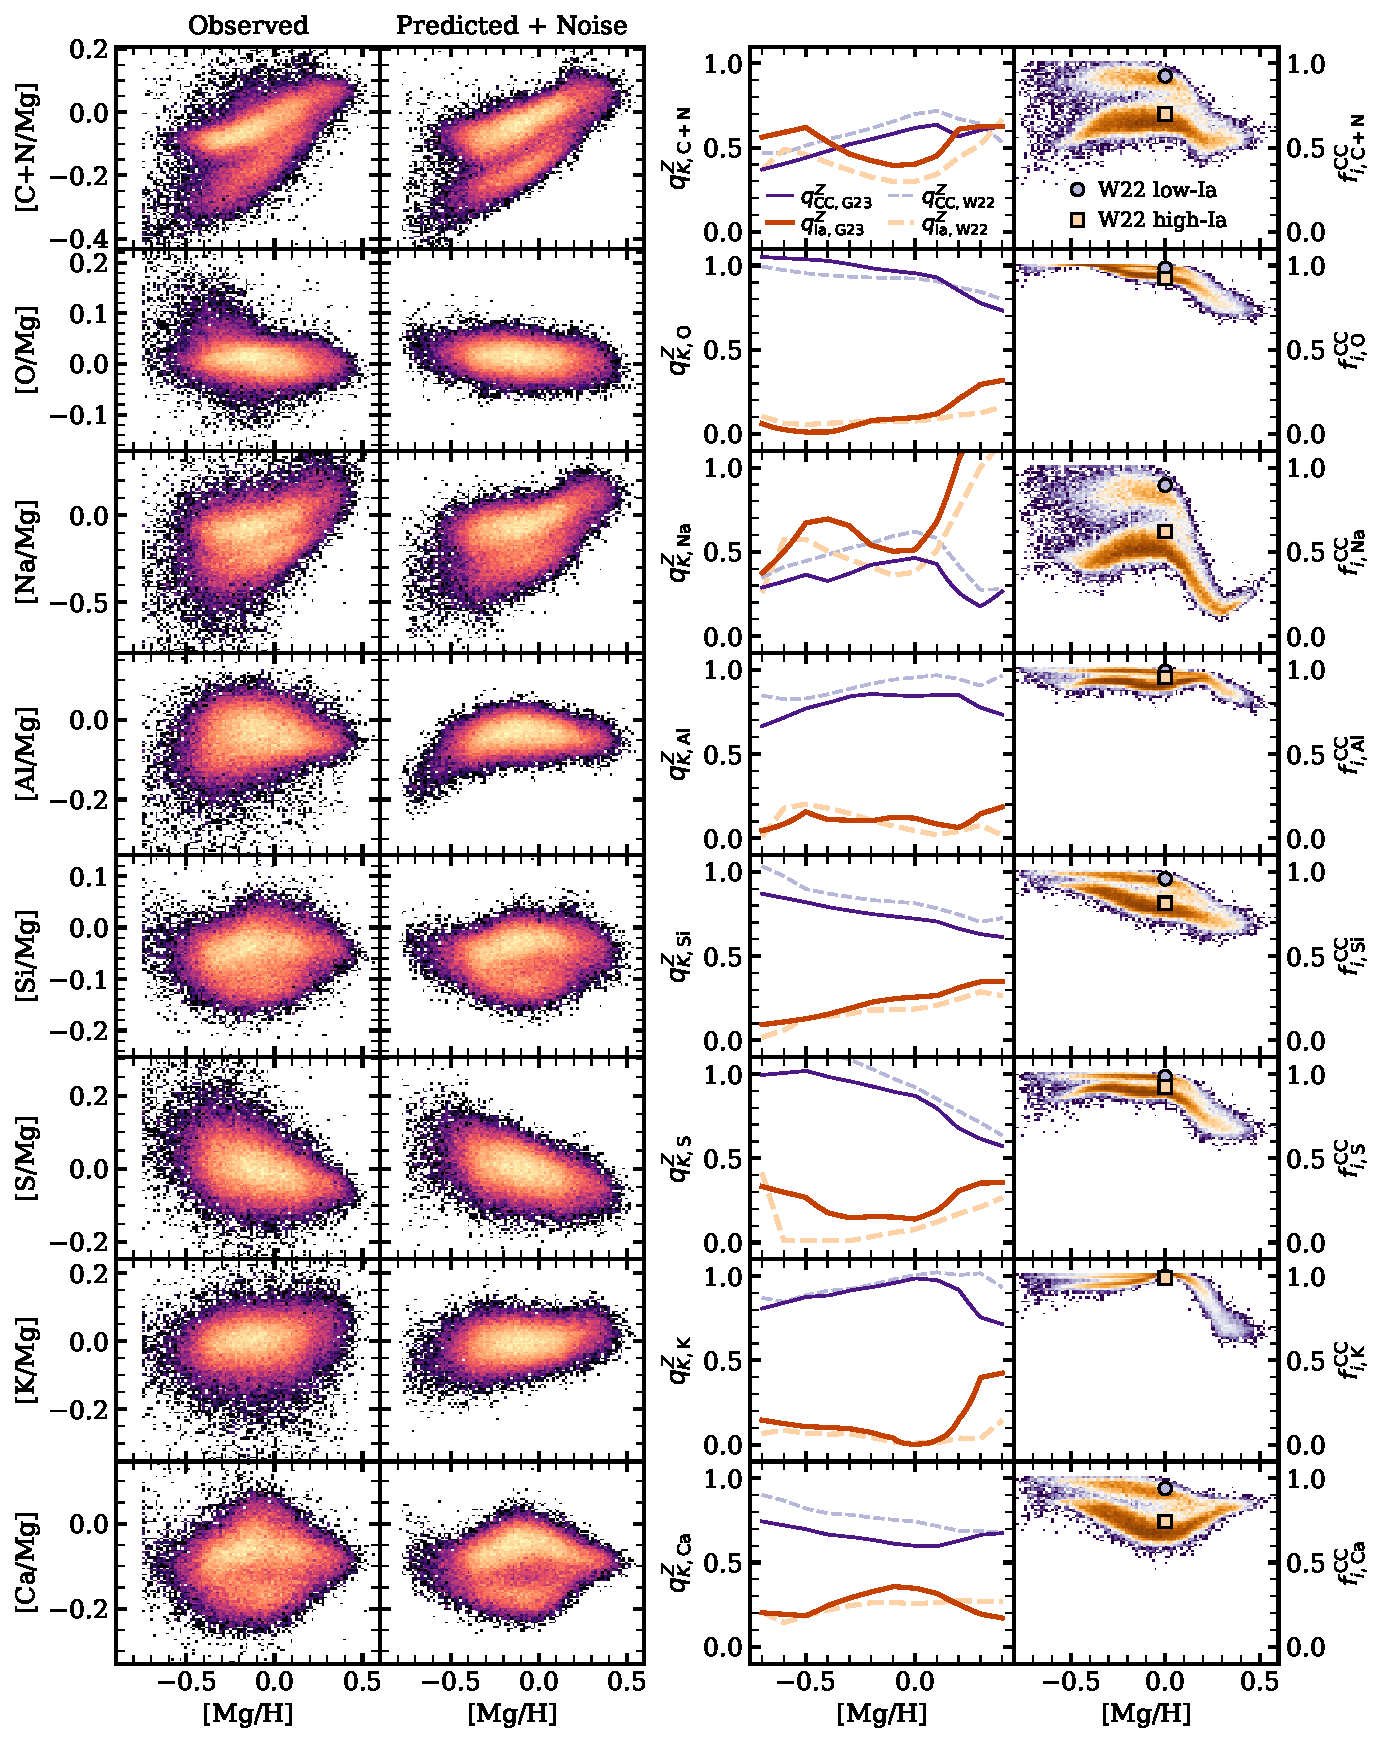
\includegraphics[width=\textwidth]{Paper/Figures/all_param1.pdf}
    \caption{Abundance distributions and Few-process model parameters for C+N, $\alpha$, and light odd-$Z$ elements. First column: observed abundance distributions in [X/Mg] vs. [Mg/H]. Second column: fiducial few-process model predicted abundance distributions in [X/Mg] vs. [Mg/H]. Third column: process vectors $\qcc$ (purple) and $\qIa$ (orange) from this work (solid, dark lines) and W22 (light, dashed lines). Fourth column: distribution of fractional contribution from the prompt process ($\fcc$) predicted by the fiducial few-process model. We plot the median $\fcc$ values of the low-Ia (orange square) and high-Ia (purple circle) populations in the solar metallicity bin from W22 for comparison.}
    \label{fig:all_param1}
\end{figure*}

\begin{figure*}[htb!]
    \centering
    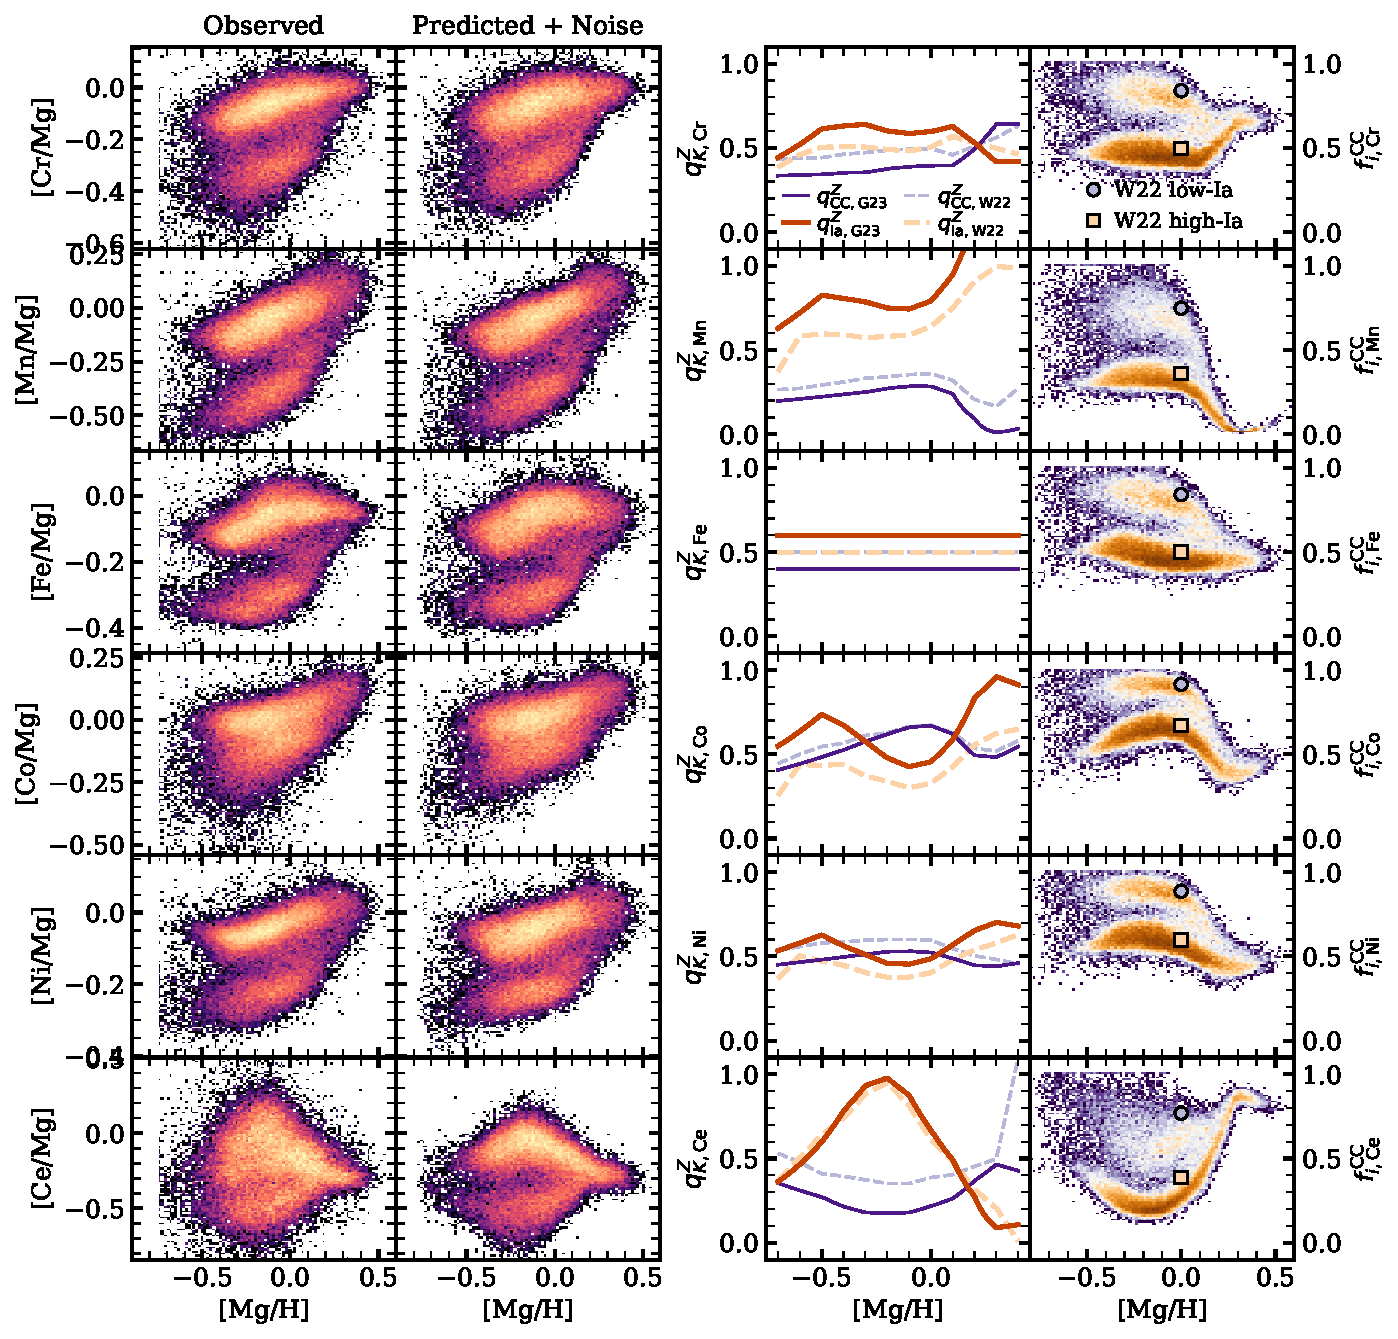
\includegraphics[width=\textwidth]{Paper/Figures/all_param2.pdf}
    \caption{Same as Figure~\ref{fig:all_param1}, but for Fe-peak elements and Ce.}
    \label{fig:all_param2}
\end{figure*}


\section{The Fiducial Model} \label{sec:fiducial}

We fit the training sample with our fiducial model of $K=2$ and $\qccFe = 0.4$ as described above. This fit produces process vectors $\qcc$ and $\qIa$ as a function of $\mgh$ for each element and process amplitudes $\Acc$ and $\AIa$ for each star. \ejg{Add sentence about the uncertainty on these values.} From the model parameters, we can calculate fractional contributions from each process as well as a full suite of predicted two-process abundances.

\subsection{Process Parameters and Fractional Contributions} \label{subsec:parameters}

We plot the process vectors as a function of $\mgh$ in the third column of Figures~\ref{fig:all_param1} and~\ref{fig:all_param2}. The process vectors inform us about the relative contribution of prompt and delayed processes to the formation of the elements, as well as the metallicity dependence of the enrichment. By definition, $\qccFe=0.4$ at all metallicities. For Fe only, we also require $\qccFe + \qIaFe = 1$, implying $\qIaFe=0.6$. No such constraints are placed on any other element. 

In the fourth column of Figures~\ref{fig:all_param1} and~\ref{fig:all_param2}, we plot the distribution of fractional contributions from the prompt process ($\fcc$) to each element, where
\begin{equation}\label{eq:fcc}
    \fcc = \frac{\Acc\qcc}{\Acc\qcc + \AIa\qIa}.
\end{equation}
We generally find that the distributions are bimodal, like the observed abundance patterns, as the high-Ia and low-Ia populations have differing fractional contributions from prompt and delayed sources.

We find that the $\alpha$-elements (O, Si, S, Ca) are best fit with $\qcc$ and $\fcc > 0.5$ at all metallicities. This is in agreement with theoretical prediction that $\alpha$-elements are dominated by prompt CCSN production \citep[e.g.][]{andrews2017}. O, a Mg-like element theoretically purely produced in prompt CCSN, shows $\fcc$ near 1 from $\mgh=-0.75$ to solar. At supersolar $\mgh$, the delayed process contributes to O production, driving the $\fcc$ value down to $\sim 0.8$ at $\mgh=0.4$. S behaves like O, with almost entirely prompt production up to solar metallicity, after which delayed enrichment contributes more significantly. Conversely, we find that Si and Ca are best fit with prompt and delayed enrichment at all metallicities, though the prompt process always dominates. For Si, the delayed process appear to increase linearly with $\mgh$, while the Ca delayed enrichment increases from $\mgh$ of $-0.75$ to $-0.1$ and then decreases from $\mgh$ of $-0.1$ to $0.5$.

The process vectors of light odd-$Z$ elements Al and K resemble those of the $\alpha$-elements, such as S. Both exhibit $\qcc$ and $\fcc$ near 1 through solar metallicity, with an increase in $\qIa$ and downturn in $\fcc$ at supersolar metallicities (especially for K). The behavior of the Na process vectors is more complex, with peaks and troughs in $\qIa$. We find that Na has the strongest contributions from the delayed process of all $\alpha$ and light odd-$Z$ elements, with $\qIa \gtrsim 0.5$ at almost all values of $\mgh$ and $\fcc < 0.3$ at $\mgh > 0$. The strong delayed contribution to Na is in agreement with findings of W22 and G22, and in tension with theoretical yields \citep[e.g.][]{andrews2017, rybizki2017}.

Unlike $\alpha$ and light odd-$Z$ elements whose delayed production is dominated by SNIa, C and N are thought to be promptly produced in CCSN with additional delayed enrichment from AGB stars \citep[e.g.][]{andrews2017}. We find that the prompt and delayed processes both contribute significantly, and nearly equally, across our stellar sample. Though theoretical N yields from AGB stars have a strong metallicity dependence \citep{karakas2010, ventura2013, cristallo2015, johnson2022}, we observe only a slight positive metallicity dependence in $\qcc$ and a shallow dip in $\qIa$. We find a population of stars with $\fcc$ near 0.9 and a population with $\fcc$ near 0.4. 

The Fe-peak elements (Cr, Mn, Fe, Co, Ni) are thought to be produced through prompt CCSN production and delayed SNIa production \citep[e.g.][]{andrews2017}. By construction, $\qccFe=0.4$ and $\qIaFe=0.6$ at all metallicities. This produces a bimodal distribution in $\fcc$ similar to that observed in abundances space. Because of our choice of $\qccFe$, only a few stars have $\fcc=1$ (see Section~\ref{subsec:qccFe}). We instead observe a population with $\fcc$ near 0.8 and a population with $\fcc$ near 0.4. The process vectors and $\fcc$ distribution for Cr and Ni strongly resemble those of Fe. All three elements have even atomic numbers. At supersolar metallicity, we find that the prompt process dominates Cr production, resulting in an upturn in $\fcc$. Conversely, Ni displays a dominant, and increasing, delayed proccess vector at supersolar metallicities. The process vectors for Mn and Co (odd atomic numbers) show a complex metallicity dependence, more resembling that of Na. Both elements display a strong delayed process, with the Mn $\qIa > 0.5$ at all metallicities and $> 1$ for $\mgh > 0.1$. Mn is the only element for which $\fcc$ decreases to 0 for $\mgh \gtrsim 0.2$. 

Finally, APOGEE DR17 reports abundances for one neutron capture element---Ce. We find that the delayed process dominates at intermediate metallicity, with $\qIa$ increasing up to $\mgh \approx -0.2$ and then decreasing to nearly 0 at $\mgh \approx 0.3$. The Ce $\fcc$ values are clustered near 0.25 around $\mgh$ of 0,2, then increase such that the abundances are almost entirely dominated by prompt enrichment at high metallicity.

In addition to process vectors, each star is fit with a prompt and delayed process amplitude, $\Acc$ and $\AIa$ respectively. All elemental abundance are used in the calculation of these amplitudes. The value of $\Acc$ traces the metallicity (specifically $\mgh$) while the ratio of $\AIa/\Acc$ traces the $\femg$ abundance. In the left panel of Figure~\ref{fig:As} we plot the distribution of $\AIa/\Acc$ vs. $\Acc$. We find a bimodal distribution, similar to the Tinsley-Wallerstein diagram ($\mgfe$ vs. $\feh$, \citealp{wallerstein1962, tinsley1979, tinsley1980}), as was also found in W22 and G22. We stress, however, that the presence of the abundance bimodality was not fed into our model, and yet it is recovered in the best-fit process amplitudes. The stars with larger $\AIa/\Acc$ values correspond to the traditional high-Ia or low-$\alpha$ population, and those with low $\AIa/\Acc$ correspond to the low-Ia or high-$\alpha$ population. While in the Tinsley-Wallerstain diagram, the two populations blend together at high-metallicity, they are more distinguishable in amplitude space. To further show this, we plot $\AIa/\Acc$ vs. $\mgh$ in the right panel of Figure~\ref{fig:As}. The high-Ia and low-Ia populations are clearly seperable through $\mgh$ of 0.4.

\begin{figure*}[htb!]
    \centering
    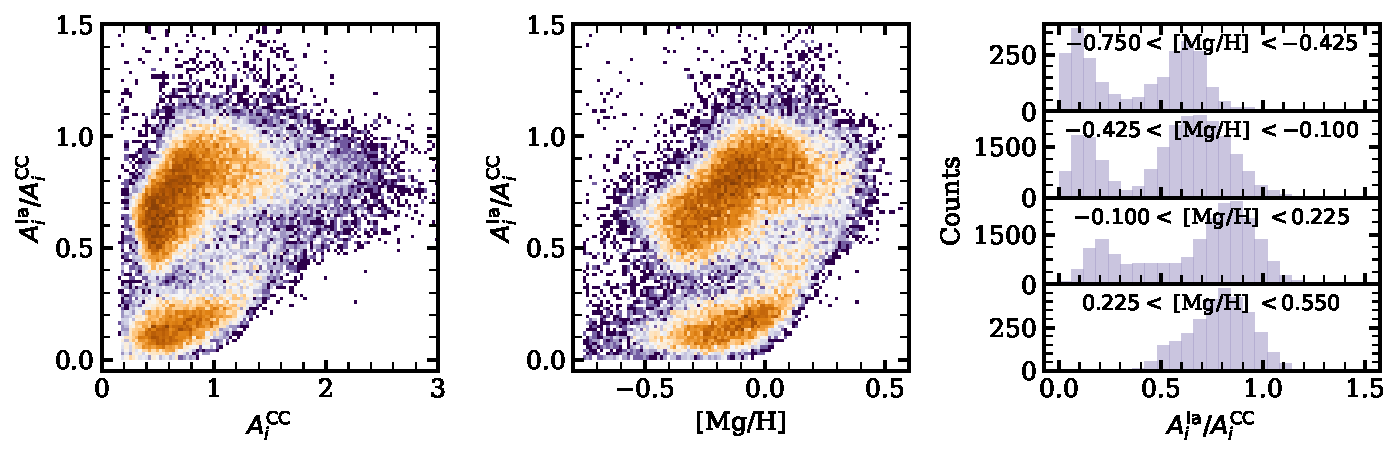
\includegraphics[width=.8\textwidth]{Paper/Figures/As.pdf}
    \caption{Left: distribution of $\AIa/\Acc$ vs. $\Acc$ for the fiducial model. Right: distribution of $\AIa/\Acc$ vs. $\mgh$. In both panels, we can clearly see the bimodality to high values of $\Acc$ and $\mgh$.}
    \label{fig:As}
\end{figure*}

\subsection{Predicted Abundances} \label{subsec:preds}

With the optimized process parameters in hand, we can use Equation~\ref{eq:xh} to calculate predicted abundances for $K=2$---the abundances our stellar population would have if the model assumptions are correct and only one prompt and one delayed process contribute. To simulate observational noise, to each abundance for each star, we add an error drawn from a Gaussian distribution with $\sigma$ equal to the reported APOGEE abundance error. In Figure~\ref{fig:all_param1} and~\ref{fig:all_param2} we plot the predicted abundances in the second columns. These distributions can be compared the the observed abundance distribution in the first columns.

Overall, the fiducial model successfully reproduces the observed abundance distributions. It is capable of capturing metalicity dependences and bimodality. The predicted abundances are not, however, able to reproduce the observed abundance scatter, especially at low metallicity. This is especially noticeable for C+N, Na, Al, K, Co, and Ce. \ejg{Add that this suggests $K>2$ or underestimated APOGEE errors?}

Amongst the $\alpha$-elements, the fiducial model successfully reproduces the near-solar [O/Mg] ratios, but does not capture the scatter above and below [O/Mg]$\approx 0$ at $\mgh\approx-0.5$ and -0.2, respectively. Similarly, the predicted abundances capture the slight negative metallicity dependence in the [S/Mg] abundances, but again fail to capture the scatter. The predicted [Si/Mg] and [Ca/Mg] abundance distributions both resemble the observed bimodal population with a small gap between the high-Ia and low-Ia populations. 

The fiducial model is also successful at reproducing the population abundance trends for the light odd-$Z$ elements, picking up the downturn in [Al/Mg] at low-$\mgh$, the upturn in [K/Mg] at high-$\mgh$, and the bimodal [Na/Mg] distribution. The predicted abundances obviously fail to capture the scatter in all light odd-$Z$ elements. Similarly, the scatter in the predicted [C+N/Mg] distribution is smaller than that of the observed. The $K=2$ model also struggles to reproduce the observed plateau at [C+N/Mg]$\approx -0.1$ and $\mgh\approx-0.5$. 

The abundance distributions of the Fe-peak elements all show strong bimodality, due in part to the substantial delayed production from SNIa. The fiducial model is able to capture the bimodality and metalicity dependence observed in Cr, Mn, Fe, Co, and Ni. We again note that the abundance scatter is slightly smaller in the predicted abundances. We also find that the [Fe/Mg] and [Ni/Mg] abundances of the high-Ia population are less dense and blurred.

The [Ce/Mg] abundance distribution is unique, displaying a rising-then-falling metallicity dependence, similar to the behavior observed in [Ba/Mg] and [La/Mg], neutron capture elements observed by GALAH (e.g. G22). This metallicity dependence is expected from the slow-neutron capture process ($s$-process) where, at low metallicity, the number of seed increases, while at high metallicity, the number of neutrons per seed becomes increasingly insufficient to produce the heavier elements \citep{gallino1998}. The $K=2$ model is able to reproduce the peaked abundance pattern, but fails to reach the high [Ce/Mg] values observed in the data. The scatter in the observed abundance distribution is much larger than in the predicted distribution, suggesting that either the $K=2$ model is insufficient or that the APOGEE scatter is underestimated.

\subsection{Comparing to W22}\label{subsec:w22}

As discussed in Sections~\ref{sec:intro} and~\ref{sec:model}, the few-process model presented in this paper is based upon the two-process model developed in W19 and W22, but with increased flexibility and no forced dependence upon the bimodality or population abundance trends. Further, the few-process model utilizes all stellar abundances in the optimization of $\Acc$ and $\AIa$, where as only Mg and Fe are used in W19 and only Mg, O, Si, Ca, Fe, and Ni in W22. 

In the fiducial few-process model, we adopt $K=2$, as in W22, but assume $\qccFe = 0.4$, 0.1 dex lower than the $\qccFe$ value assumed in W22. In practice, this moves the implied ``pure'' CCSN enrichment plateau from $\femg=-0.3$ to $\femg=-0.4$ (though W22 plateau value is determined \textit{after} they apply a global offset of +0.05 to all $\femg$ abundances). Because our model is non-negative, it requires a lower $\qccFe$ and thus lower plateau value to correctly model the stars on the $\femg$ plateau, where as W22 assigns stars with $\femg < -0.3$ negative $\AIa$ values.

While our stellar samples and model assumptions differ, we plot the W22 $\qcc$ and $\qIa$ vectors as well as the W22 median $\fcc$ values of their high-Ia and low-Ia populations at $\mgh=0$ in columns three and four, respectively, of Figures~\ref{fig:all_param1} and~\ref{fig:all_param2} for comparison to the few-process model parameters. 

Amongst the process vectors, we generally observe similar behavior between our model and W22. Our $\qIa$ vectors tend to be $\sim 0.1$ greater than those of W22 for elements with significant delayed contributions because of our differing $\qccFe$ assumptions. The metallicity dependencies agree for most elements, with small variations at the high-$\mgh$ end for O, Al, K, and Ce. We also see good agreement between the two models' solar $\fcc$ values, with the W22 points slightly offset to larger values for elements with significant delayed contributions, again because of our differing $\qccFe$ assumptions.

To compare the accuracy of the models' abilities to reproduce the observed abundances, we identify a subset of $\sim 23,000$ stars in our training sample and the W22 sample. We calculate the few-process and two-process predicted abundances for each star, then determine the $\chi^2$ value of the fits for each star (summing over the elements) and for each element (summing over the stars). We plot the cumulative stellar $\log(\chi^2)$ distribution and the total $\chi^2$ for each element in the right and left panels, respectively, of Figure~\ref{fig:comp_w22}. It is important to note that in the calculation of the W22 model residuals, we do not apply the temperature correction discussed in Section 5.1 of W22. We find that, overall, the $\log(\chi^2)$ decreases between the W22 two-process model and our few-process model, an indication that we better predict the stellar abundances. When we look at each element individually, we find that we better predict C+N, Na, K, Ni, Mn, Co, and Ce, with major improvements to C+N and Mn. Our fiducial model is significantly worse at predicting Mg, Ca, and Fe than the W22 model, all elements that W22 fit to.

\begin{figure*}[htb!]
    \centering
    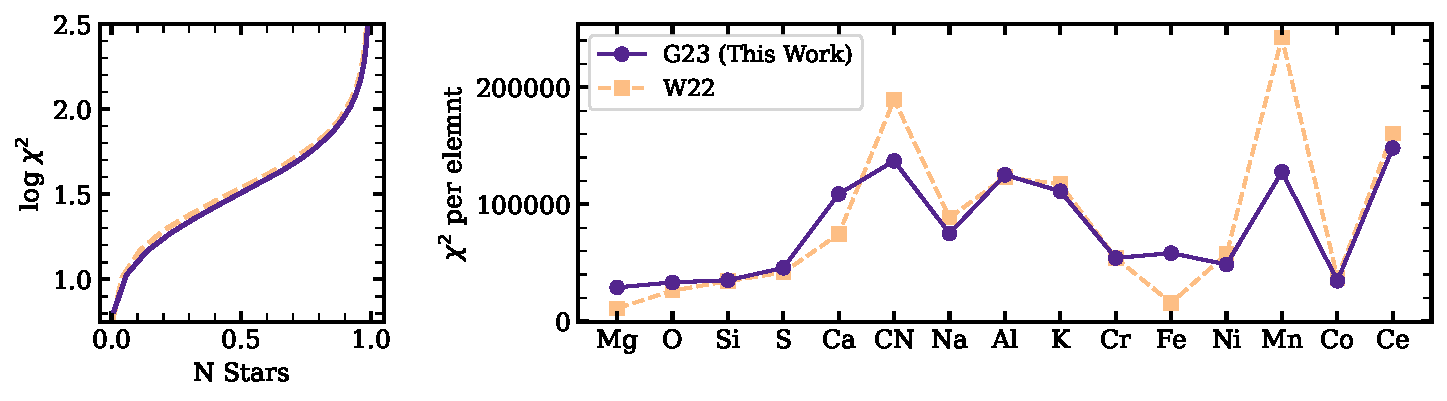
\includegraphics[width=\textwidth]{Paper/Figures/comp_w22.pdf}
    \caption{Left: cumulative distribution of $\log \chi^2$ for W22 (dashed orange line) and our fiducial model (solid purple line). Right: $\chi^2$ per element for the same model fits. }
    \label{fig:qs}
\end{figure*}

In this comparison, it is important to note our fiducial model is fit to a larger stellar sample that spans a wider range of $\teff$ and $\logg$ than the W22 sample. If we repeat our analysis on the W22 stellar sample with $\qccFe=0.5$ we almost perfectly recover the W22 process vectors, with small deviations at $\mgh>0.1$, and more substantially improve upon the stellar and elemental $\chi^2$ values. Most notably, the few-process model is better able to predict the abundances of stars with $\mgh>0$, where the high-Ia and low-Ia sequences blend together and the W22 division of high-Ia and low-Ia stars may be incorrect. \ejg{Would it be worth adding an appendix on this?}

\section{Variations from the Fiducial Model} \label{sec:variations}

\subsection{Choice of $\qccFe$} \label{subsec:fcc}

\ejg{I think I have too many plots in this section....}

While the few-process model is flexible, it still requires us to make assumptions in order for the parameters to converge. Specifically, it requires an element with ``known'' $\qcc$ and an element with known $\qIa$ to constrain each process and to break degeneracies. For the prompt process, we ground our assumption in the nucleosynthetic fact (\ejg{change wording}) that Mg is a pure CCSN element \citep[e.g.,][]{andrews2017}. Unfortunately, there is no comparable pure SNIa element, nor is there an element for which we know the relative CCSN/SNIa ratio. In order to regularize the delayed process, we choose to fix the Fe process vectors, making unsubstantiated assumptions about Fe enrichment. 

In the fiducial model, we choose $\qccFe = 0.4$ as this parameter choice is able to reproduce the observed [Fe/Mg] vs. [Mg/H] abundance distribution, as discussed in Section~\ref{subsec:parameters}. This choice impacts the predicted abundances as well as the implied $\fcc$ values of each star. In this section, we explore the implications of different $\qccFe$ assumptions, varying the zero point and metallicity dependence ($\dqccFe$). Because our model is non-negative, the choice of $\qccFe$ set the minimum [Fe/Mg] value attainable by our model ($\log_{10}(\qccFe)$). Under the $K=2$ few-process model, any observed [Fe/Mg] abundance below this boundary can only be explained by noise. In Figure~\ref{fig:qccFe_FeMg}, we plot the minimum [Fe/Mg] as a function of $\mgh$ for the $\qccFe$ and $\dqccFe$ parameters we explore. With a $\dqccFe=0.0$, we choose $\qccFe=0.5$ (the W22 value), 0.45 (approximate plateau value at $\mgh=-0.75$), 0.4 (the fiducial value that skirts the edge of the distribution), and 0.35 (captures almost all stars). With a $\dqccFe=0.15$, which roughly matches the slope of the low-Ia sequence at intermediate metallicity, we choose $\qccFe=0.5$ (passes through the center of the low-Ia density), 0.4 (skirts the edge of the distribution), 0.3 (captures almost all stars)

\begin{figure*}[htb!]
    \centering
    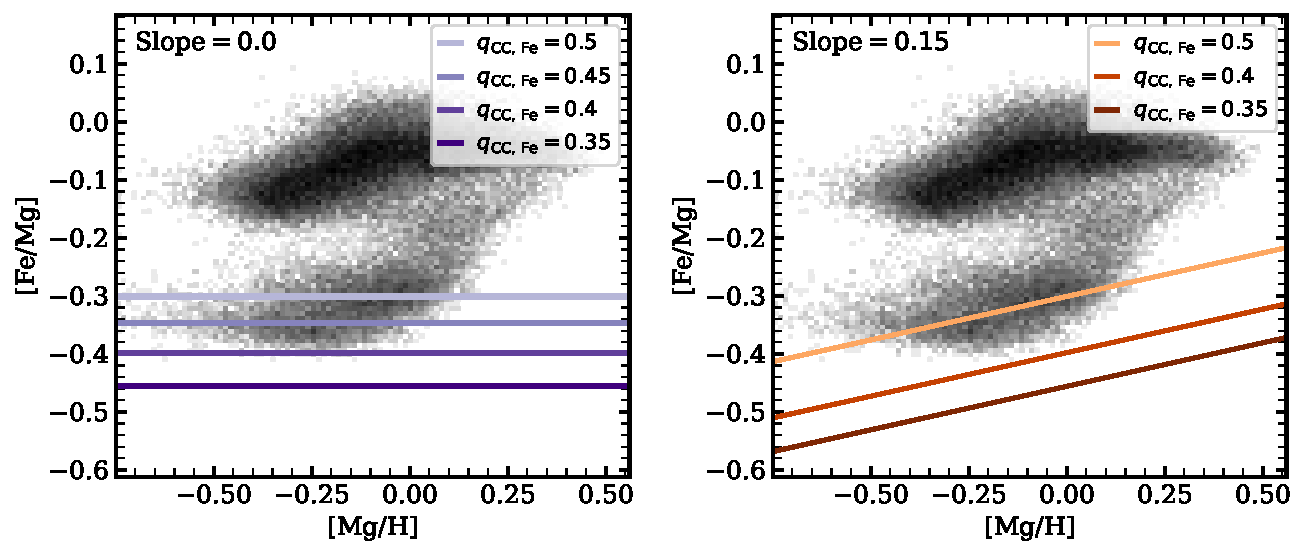
\includegraphics[width=\textwidth]{Paper/Figures/qccFe_FeMg.pdf}
    \caption{Minimum [Fe/Mg] value attainable for $\qccFe$ and $\dqccFe$ assumptions. Left: For $\dqccFe=0$ with $\qccFe=0.5$, 0.45, 0.4, and 0.3 (light to dark purple). Right: For $\dqccFe=0.15$ with $\qccFe=0.5$, 0.4, 0.35 (light to dark orange).}
    \label{fig:qccFe_FeMg}
\end{figure*}

We repeat the optimization of the few-process model with $K=2$ and these $\qccFe$ assumptions, as described in Section~\ref{sec:model}. In Figure~\ref{fig:qccFe_FeMgpred}, we plot the predicted abundance distributions (including APOGEE noise), as in the second column of Figures~\ref{fig:all_param1} and ~\ref{fig:all_param2}. We do not plot the predictions for the fiducial model ($\qccFe=0.4$, $\dqccFe=0.0$), as these have been shown in Section~\ref{subsec:preds}. Both models with $\qccFe=0.5$ fail to reproduce the shape and width of the low-Ia abundance distribution. They instead predict a much thinner sequence that is flat for $\dqccFe=0.0$ or slightly inclined for $\dqccFe=0.15$. The model with $\qccFe=0.45$ and $\dqccFe=0.0$ is better, but still predicts a low-Ia abundance distribution that is too thin, flat, and dense. The other four models ($\qccFe=0.35$ and $\qccFe=0.4$ with $\dqccFe=0.0$ and $\dqccFe=0.15$) predict an abundance distribution that strongly resembles the observed. There are minor differences at the low [Fe/Mg] and low-metallicity end, but it is difficult to tell by eye which model is best.

\begin{figure*}[htb!]
    \centering
    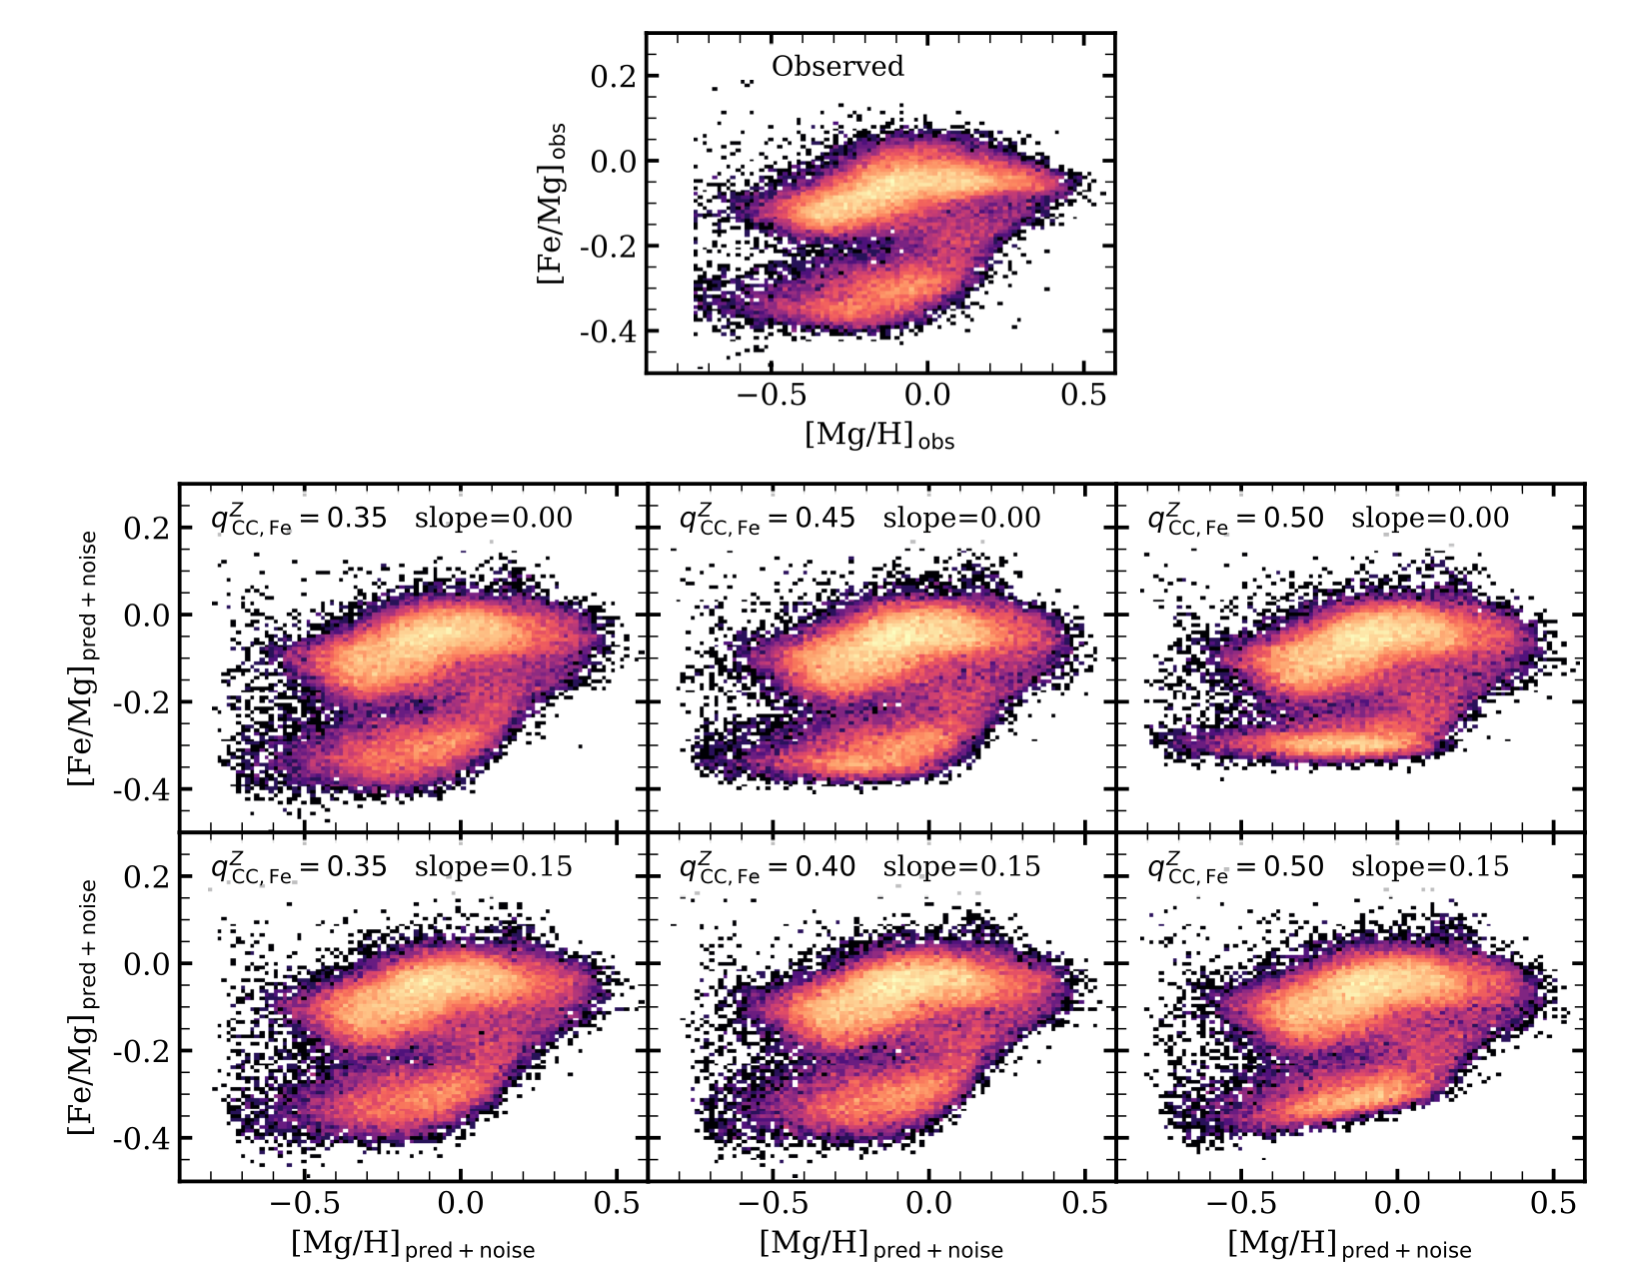
\includegraphics[width=\textwidth]{Paper/Figures/qccFe_FeMgpred.pdf}
    \caption{Predicted [Fe/Mg] vs. [Mg/H] abundance distributions for models with $\dqccFe=0.0$ (top row) and $\dqccFe=0.15$ (bottom row). The $\qccFe$ value increase from left to right from 0.35 to 0.5. $\qccFe$ and $\dqccFe$ parameters are listed in each panel.}
    \label{fig:qccFe_FeMgpred}
\end{figure*}

To better assess the models' goodness of fit, we calculate the average $\chi^2$ value per star for each case and plot the results in Figure~\ref{fig:qccFe_chi2}. The models with $\qccFe$ of 0.5 or 0.45, regardless of $\dqccFe$, have an average $\chi^2$ per star $>90$ while the models with $\qccFe$ of 0.4 and 0.35 have an average $\chi^2$ per star $< 55$. In both the metallicity independent and metalicity dependent models, the models with $\qccFe=0.4$ have the lowest average $\chi^2$ per star, by 0.13 and 0.8 respectively. Of the seven models explored here, the case with $\qccFe=0.4$ and $\dqccFe=0.15$ has the lowest average $\chi^2$ per star of 54.47, indicating that the stellar abundances are best fit by a metallicity dependent CCSN process. 

\begin{figure*}[htb!]
    \centering
    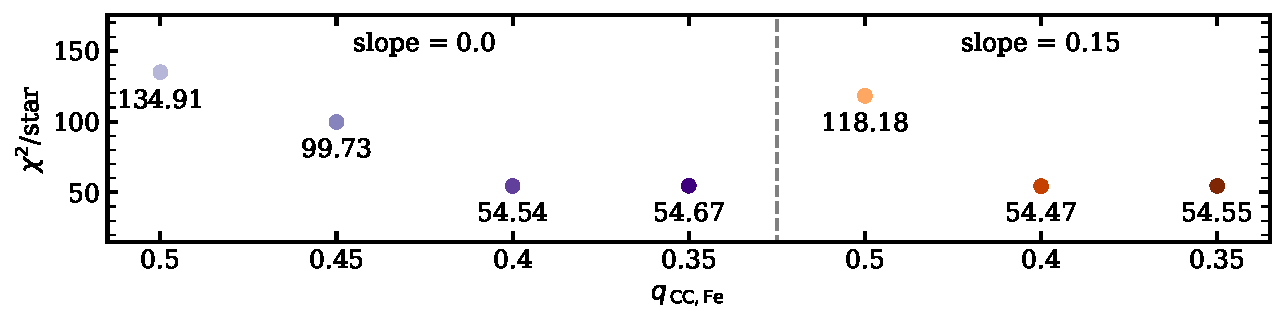
\includegraphics[width=\textwidth]{Paper/Figures/qccFe_chi2.pdf}
    \caption{Average $\chi^2$ per star for few-process models with a range of $\qccFe$ and $\dqccFe$ values. \ejg{Maybe this should just be a table.}}
    \label{fig:qccFe_chi2}
\end{figure*}

Though the $\qccFe= 0.4$ and 0.35 are similar in terms of their goodness of fit, their nucleosynthesis implications are more significant. In Figure~\ref{fig:qccFe_fcc}, we plot the median value of $\fcc$ (Equation~\ref{eq:fcc}) for the low-Ia population (as defined in W22 \ejg{need to add this definition}) at solar metallicity ($-0.05 < \mgh < 0.05$). We only show the $\fcc$ values for the models with $\dqccFe=0.0$ as the solar metallicity $\fcc$ values for the models with $\dqccFe=0.15$ are almost identical for matching values of $\qccFe$.

In Figure~\ref{fig:qccFe_fcc}, we find that the choice of $\qccFe$ has little impact on the $\fcc$ of elements dominated by CCSN enrichment (e.g. O, S, Al, K). As the delayed contribution increases, the elemental $\fcc$ values decrease more significantly with decreasing $\qccFe$. The choice of $\qccFe$ most impacts the $\fcc$ values for Na, Cr, Fe, Mn, and Ce, with the $\fcc$ for Mn decreasing from 0.42 for $\qccFe=0.5$ to 0.22 for $\qccFe=0.35$. Because the $\qccFe$ value sets the ``pure CCSN'' plateau, a lower $\qccFe$ model implies a lower $\fcc$ value. 

While the high $\qccFe$ model can likely be ruled out due to poorness of fit, the true $\qccFe$ value and its metallicity dependence are unknown. It is therefore important not to over-interpret the specific $\fcc$ values of a given model, or to include error bars based on a range of reasonable $\qccFe$ assumptions. The $\fcc$ parameter can provide qualitative descriptions of which elements have more or less prompt/delayed enrichment, but the exact values are uncertain by up to XXX\%

\begin{figure*}[htb!]
    \centering
    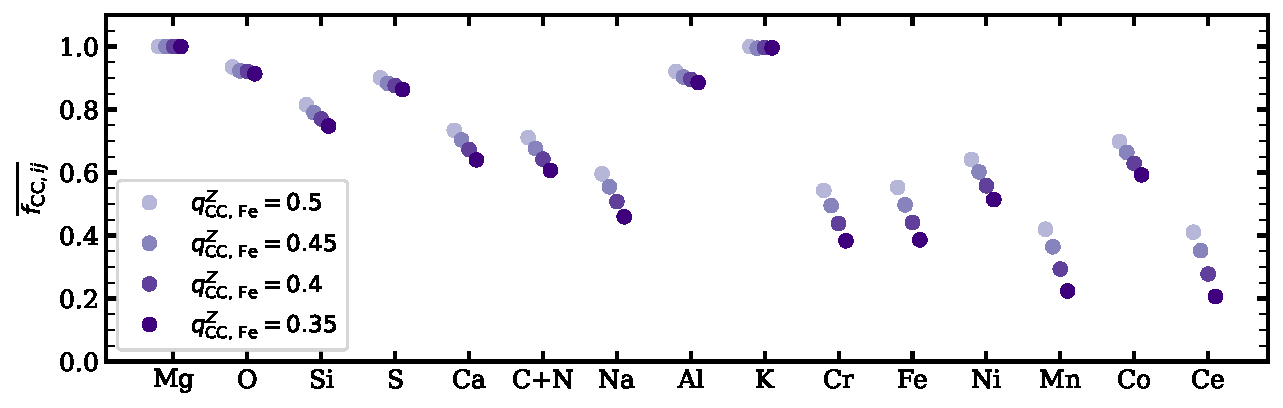
\includegraphics[width=\textwidth]{Paper/Figures/qccFe_fcc.pdf}
    \caption{Elemental median values of $\fcc$ at solar metallicity for the low-Ia population for few-process models with $\qccFe=0.35$ (darkest purple) to 0.5 (lightest purple) and $\dqccFe=0.0$. \ejg{Add legend!}}
    \label{fig:qccFe_fcc}
\end{figure*}

\ejg{Maybe a run where we turn down the regularization on qcc Fe and see what it picks? Update: tried this and it failed to converge}

\subsection{Increasing to $K=4$} \label{subsec:k=4}

\section{Application to a Broader Data Sample} \label{sec:results_broad}

\subsection{Testing Sample}

\ejg{I think this should be moved to the end for an entire section on the testing sample.}

Beyond the training sample presented above, we are also interested in the Few-Process model's implications for a wider sample of data. In Section X, we argue that the Few-Process model produces high signal-to-noise abundance labels, as it uses all elements for all stars to learn the process parameters. These high SNR labels are useful for XYZ and allow us to understand what the abundance patterns \textit{would} look like if our model assumptions are correct. To provide the community with a large catalog of such labels, we apply the fiducial Few-Process model to the APOGEE RC and RGB sample, defined by the following cuts:
\itemsep0em
\begin{itemize}
    \item \texttt{STAR\_BAD} = 0
    \item \texttt{NO\_ASPCAP\_RESULT} = 0
    \item \texttt{EXTRATARG} = 0
    \item $\logg =  0 - 3.5$ dex
    \item $\teff = 3200-6000$ K
    \item $\mgh > -0.75$
\end{itemize}
with the upper $\teff$ limit and $\logg$ used as RGB classifiers in \citet{jonsson2020}. Our full sample includes 227,601 stars. We again only analyze [X/Mg] abundances for stars where the [X/Fe] value is unflagged, most drastically reducing the sample size to 195,117 for Ce. 

\begin{figure*}[htb!]
    \centering
    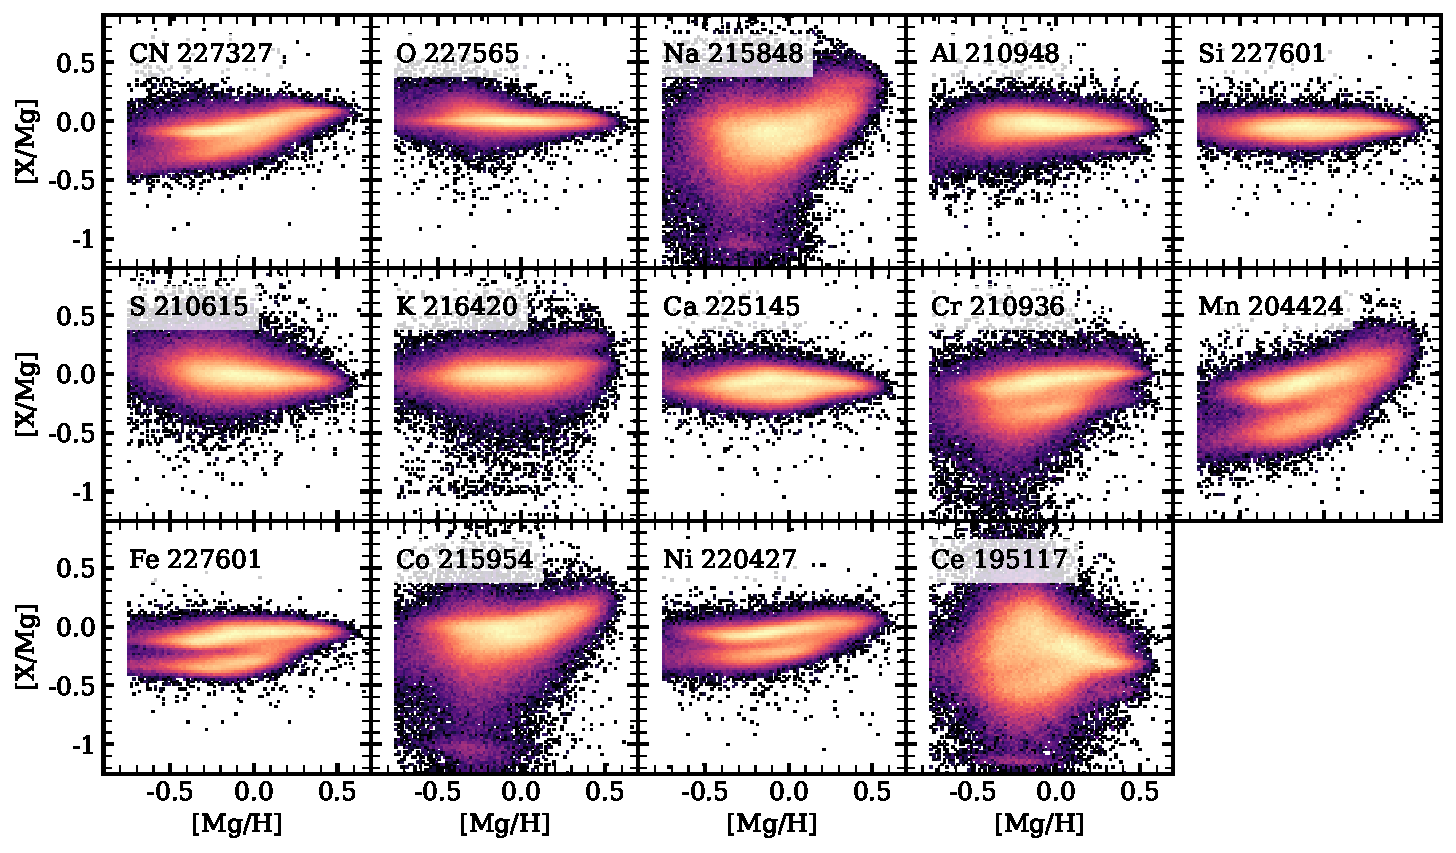
\includegraphics[width=\textwidth]{Figures/xmg_test.pdf}
    \caption{Stellar abundance distributions for our expanded RGB and RC sample. The number in the top right corner indicates the number of stars used in the analysis of that element. Elements are ordered by atomic number. No zero-point offsets have been applied.}
    \label{fig:exp_xmg}
\end{figure*}

We plot the distribution of abundances in [X/Mg] vs. [Mg/H] for the testing sample in Figure~\ref{fig:exp_xmg}. The expansion of the data sample does introduce abundance systematics that our training sample sought to exclude. As discussed in \citet{jonsson2020} and \citet{griffith2021a}, APOGEE DR16 and DR17 suffer from poorly understood abundance artifacts, such as a ``finger'' in [$\alpha$/M] and low-[X/Fe] banding in elements such as Al and Ni. In our expanded data set, we observe potential abundance artifacts in Na, Al, K, Cr, Co, and Ce, as well as larger scatter for all elements.  



\begin{itemize}
    \item Look at residuals from the K=2 fit, are there elements with correlated residuals? Are they the same as in W22? 
    \item show results for adding 3rd and 4th process to the data
\end{itemize}


\section{Summary}\label{sec:summary}

Notes

\begin{itemize}
    \item What is the connection between this model and latent variable models of machine learning
    \item Casual inferences - which abundances are caused by the Mg abundance and which are not (statistician perspective)
    \item Implications of differences at high metallicity
    \item Observational motivation for additional processes, what elements are critical for spectral surveys to observe
    \item Why this version of the 2 process model is more flexible than W22
    \item two dimensional doesn't mean there are two processes, things are just getting mixed down to two dimensions  - maybe two d because radius and age, if true then our labels should predict age and radius 
    \item our 2 dimentionality is not defined by the bimodality like W22 is
    \item why k=2 is a good fit to this data, all the different ways we could get K=2 - young open clusters don't fit the model is a blow against the view
\end{itemize}

\section{Acknowledgements}
It is a pleasure to thank
  Soledad Villar (JHU)
for valuable discussions.
This project benefited enormously from the Python package \texttt{jax} \citep{jax}.
E.J.G. is supported by an NSF Astronomy and Astrophysics Postdoctoral Fellowship under award AST-2202135.
CU Boulder Research Computing services and staff

% \software{Matplotlib \citep{hunter2007}, NumPy \citep{harris2020}, Pandas \citep{pandasa, pandasb}, Astropy \citep{astropy2013, astropy2018, astropy2022}, astroNN \citep{bovy2017}, EXOFASTv2 \citep{eastman2013, eastman2019}, iSpec \citep{blanco2014, blanco2019}, MOOG \citep{sneden1973}, galpy \citep{bovy2015, mackereth2018}}, jax \citep{jax}

\bibliography{sample631}{}
\bibliographystyle{aasjournal}

\end{document}

